\documentclass[a4paper,11pt]{article}
\usepackage{graphicx}
\usepackage{esvect}
\usepackage{subcaption}
\usepackage{listings}
\usepackage[top=0.75in, bottom=0.75in, left=0.6in, right=0.6in]{geometry}

\title{AE 625 - Particles Methods for Fluid Flow Simulation \\ Vortex sheet roll up}
\author{Chillapalli Jyothi Durga Prasad - 140010042 }
\date{21 August 2017}

\usepackage{color}
 

\begin{document}
\maketitle


\tableofcontents
\listoffigures


\newpage
\section{Consider a single blob placed at the origin with circulation 1 $m^2/s$. Assume a kinematic viscosity of 0.1 $m^2/s$. Calculate the vorticity distribution under pure diffusion after a time of 1 second.}

\indent Use increasing number of vortices to do this. Compare the result with the exact solution. In order to do this, interpolate the vorticity onto a mesh using a simple linear remeshing strategy. You can easily derive the expression for this considering a generic point at a coordinate (x, y) and the linear interpolation kernel we discussed in class. Recall that the exact solution for a point vortex at the origin is exactly the heat kernel as I had written down in class.\\

\begin{centering}
    $$\frac{1}{4 \pi \nu t} e^{\frac{-r^2}{4 \nu t}}$$
\end{centering}


\textbf{Results:}\\

The vortex blob is divided to smaller blobs and the no of division per blob is fixed at the start of the simulation. The final number of blobs depend on the no of division and minimum circulation strength further which there is no division.\\


The diffusion is simulated through a random walk process whose displacement for time step $\zeta$ is governed by a normal distribution with mean 0 and standard deviation $\sqrt{2\nu t}$. \\

The diffused particles are then interpolated to mesh using simple linear remeshing strategy.\\

The contribution to three nearest grid points are

\begin{centering}
    $$\Gamma _{1} = \Gamma \frac{x(x - 1)}{2}$$\\
    $$\Gamma _{2} = \Gamma (1 - x^{2})$$\\
    $$\Gamma _{1} = \Gamma \frac{x(x + 1)}{2}$$\\
\end{centering}


we know that vorticity at some location $\vec{r}$ is\\ 
\begin{centering}
    $$\omega(\vec{r}) = \sum_{j = 0}^{N} \Gamma_{j} f_{\delta}(\vec{r} - \vec{r}_{j})$$\\
\end{centering}

here $f_{\delta}(\vec{r} - \vec{r}_{j})$ is a dirac-delta function.\\

The exact solution for a diffused vortex blob is given by:

\begin{centering}
    $$\omega (x_{0},y_{0}) = \frac{1}{4 \pi \nu t} \int_{y_{0} - 0.5dy}^{y_{0} + 0.5dy}\int_{x_{0} - 0.5dx}^{x_{0} + 0.5dx} e^{-\frac{(x^{2} + y^{2})}{4 \nu t}} \Gamma _{0} dx dy$$
    
    
\end{centering}

\begin{figure}[h]
    \centering
    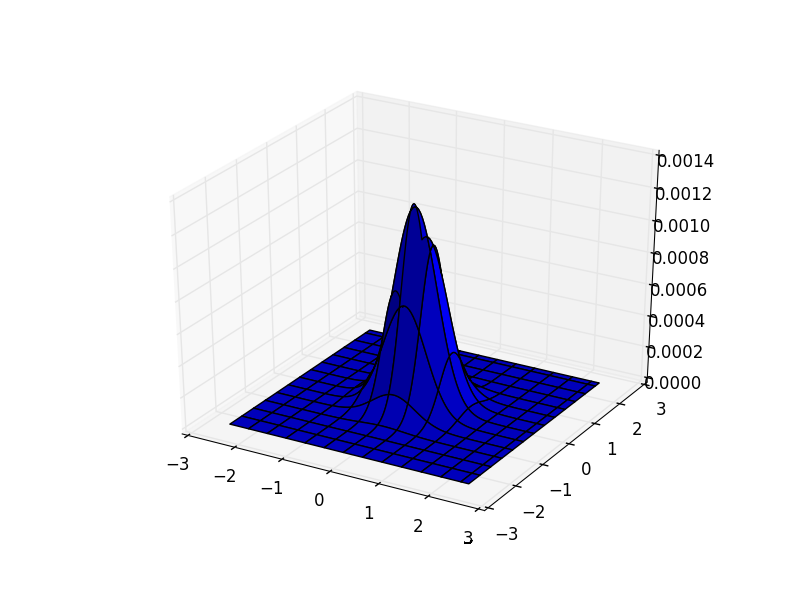
\includegraphics[width=.8\linewidth]{Exact_solution_of_diffusion_for_1_sec.png}
    \caption{Exact solution of diffused vorticity after 1 sec}
    \label{fig:ex}    
\end{figure}

\begin{figure}[h]
	\centering
	\begin{subfigure}[h]{.5\textwidth}
  		\centering
  		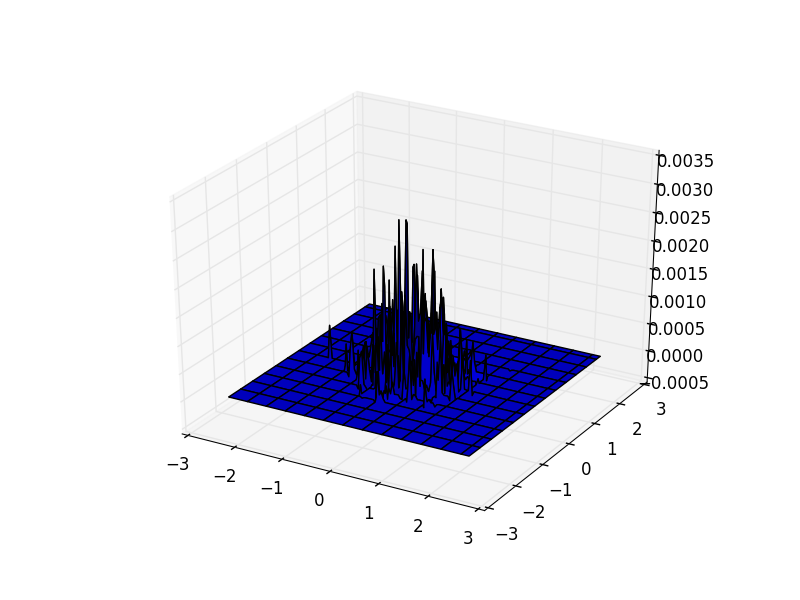
\includegraphics[width=.8\linewidth]{vorticity_distribution_for_1600_particles.png }
  		\caption{vorticity distribution for 1600 particles }
  		\label{fig:16}
	\end{subfigure}
	\begin{subfigure}[h]{.5\textwidth}
  		\centering
  		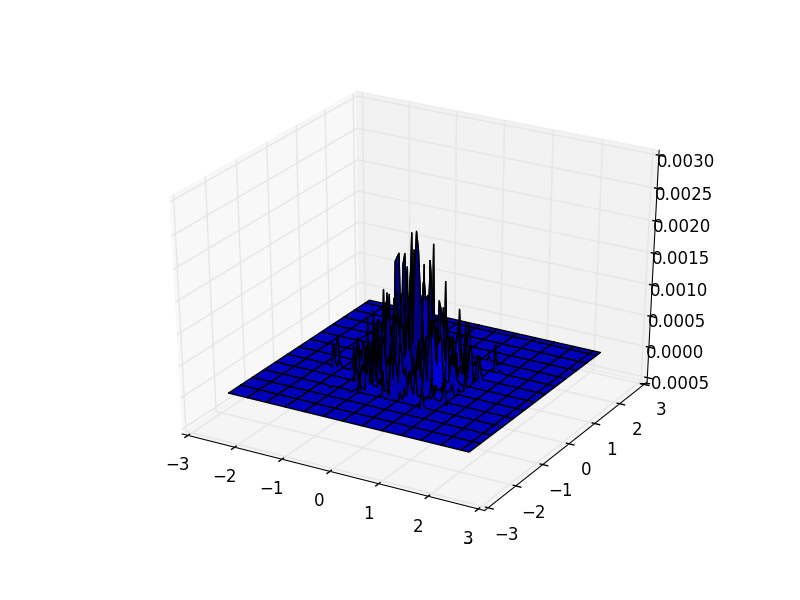
\includegraphics[width=.8\linewidth]{vorticity_distribution_for_2500_particles.png}
  		\caption{vorticity distribution for 2500 particles}
  		\label{fig:25}
	\end{subfigure}%
	\label{fig:Question 1a}
  \caption{vorticity distribution for 1600 \& 2500 particles}
\end{figure}

\begin{figure}[h]
	\centering
	\begin{subfigure}[h]{.5\textwidth}
  		\centering
  		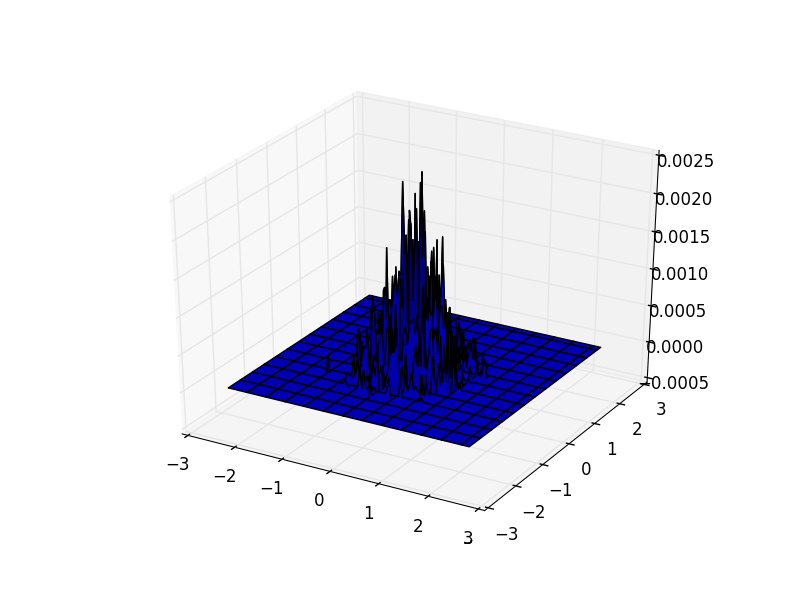
\includegraphics[width=.8\linewidth]{vorticity_distribution_for_3600_particles.png}
  		\caption{vorticity distribution for 3600 particles}
  		\label{fig:36}
	\end{subfigure}
	\begin{subfigure}[h]{.5\textwidth}
  		\centering
  		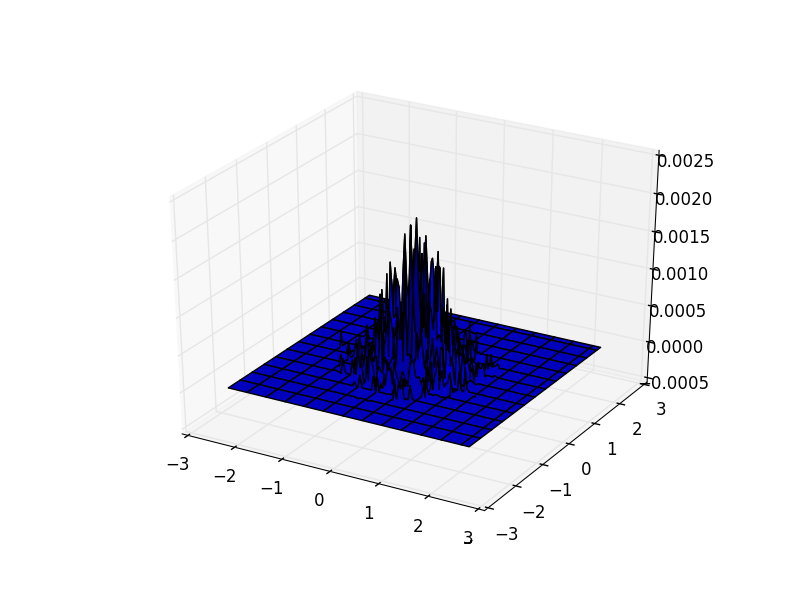
\includegraphics[width=.8\linewidth]{vorticity_distribution_for_4900_particles.png}
  		\caption{vorticity distribution for 4900 particles}
  		\label{fig:49}
	\end{subfigure}%
	\label{fig:Question 1a}
  \caption{vorticity distribution for 3600 \& 4900 particles}
\end{figure}

\begin{figure}[h]
	\centering
	\begin{subfigure}[h]{.5\textwidth}
  		\centering
  		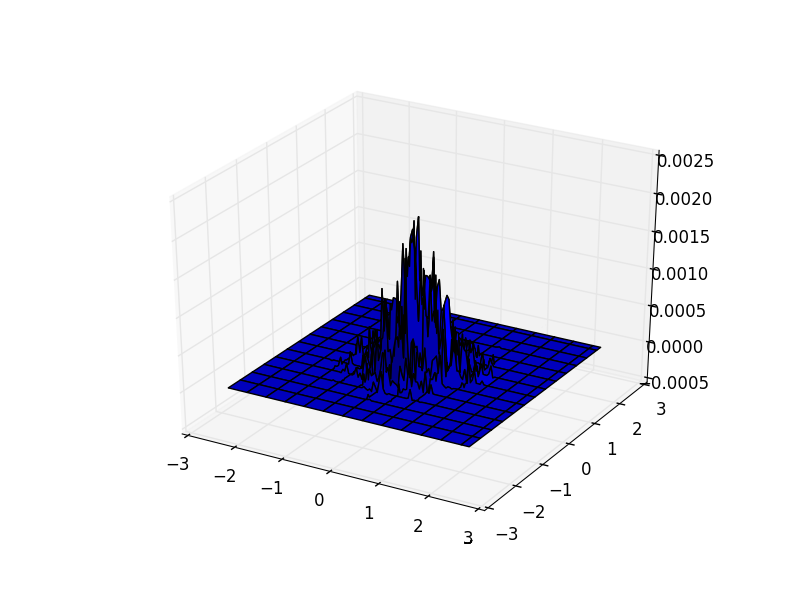
\includegraphics[width=.8\linewidth]{vorticity_distribution_for_6400_particles.png}
  		\caption{vorticity distribution for 6400 particles}
  		\label{fig:64}
	\end{subfigure}
	\begin{subfigure}[h]{.5\textwidth}
  		\centering
  		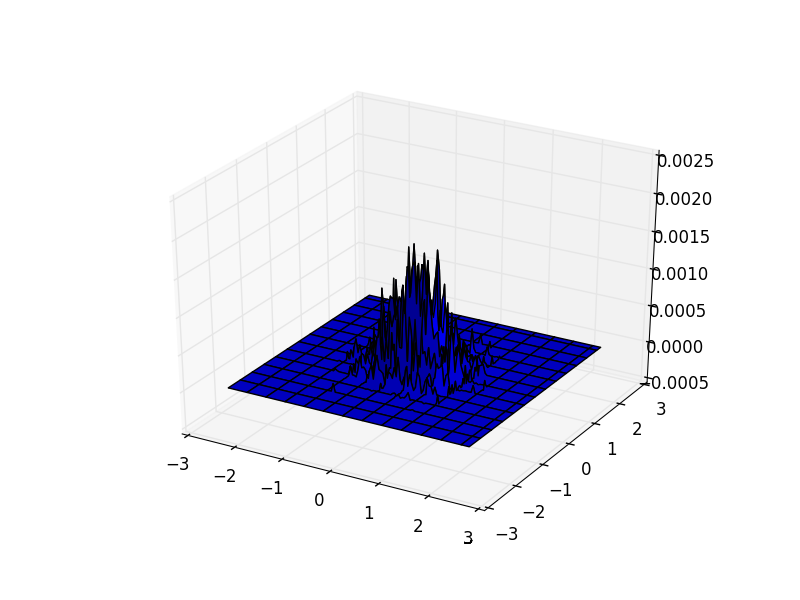
\includegraphics[width=.8\linewidth]{vorticity_distribution_for_8000_particles.png}
  		\caption{vorticity distribution for 8000 particles}
  		\label{fig:80}
	\end{subfigure}
	\label{fig:Question 1a}
  \caption{vorticity distribution for 3600 \& 8000 particles}
\end{figure}

\begin{figure}[h]
	\centering
	\begin{subfigure}[h]{.5\textwidth}
  		\centering
  		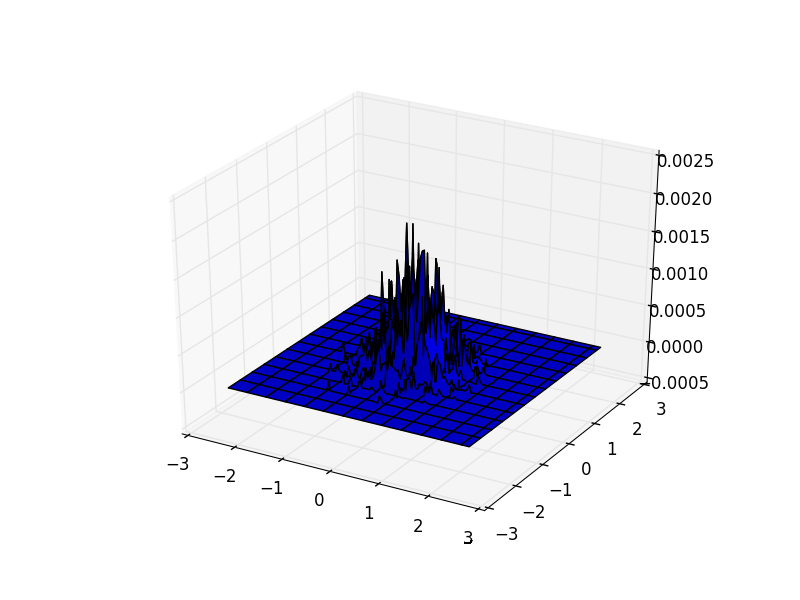
\includegraphics[width=.8\linewidth]{vorticity_distribution_for_8100_particles.png}
  		\caption{vorticity distribution for 8100 particles}
  		\label{fig:81}
	\end{subfigure}%
	\begin{subfigure}[h]{.5\textwidth}
  		\centering
  		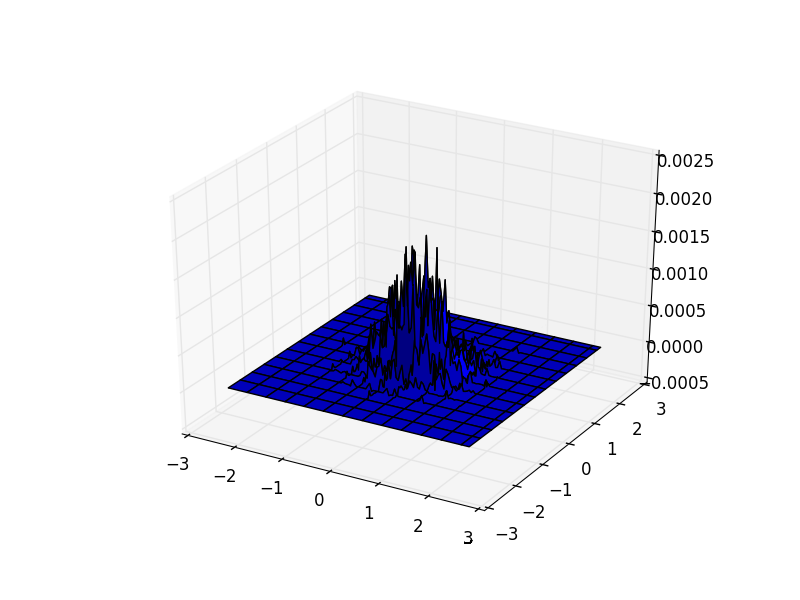
\includegraphics[width=.8\linewidth]{vorticity_distribution_for_10000_particles.png}
  		\caption{vorticity distribution for 10000 particles}
  		\label{fig:100}
	\end{subfigure}
	\label{fig:Question 1a}
  \caption{vorticity distribution for 8100 \& 10000 particles}

\end{figure}

\begin{figure}[h]
	\centering
	\begin{subfigure}[h]{.5\textwidth}
  		\centering
  		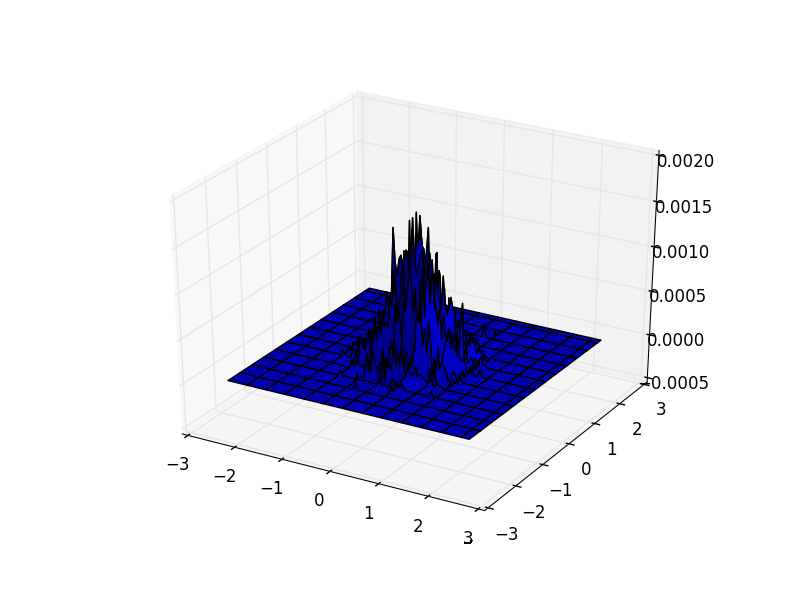
\includegraphics[width=.8\linewidth]{vorticity_distribution_for_12100_particles.png}
  		\caption{vorticity distribution for 12100 particles}
  		\label{fig:121}
	\end{subfigure}%
	\begin{subfigure}[h]{.5\textwidth}
  		\centering
  		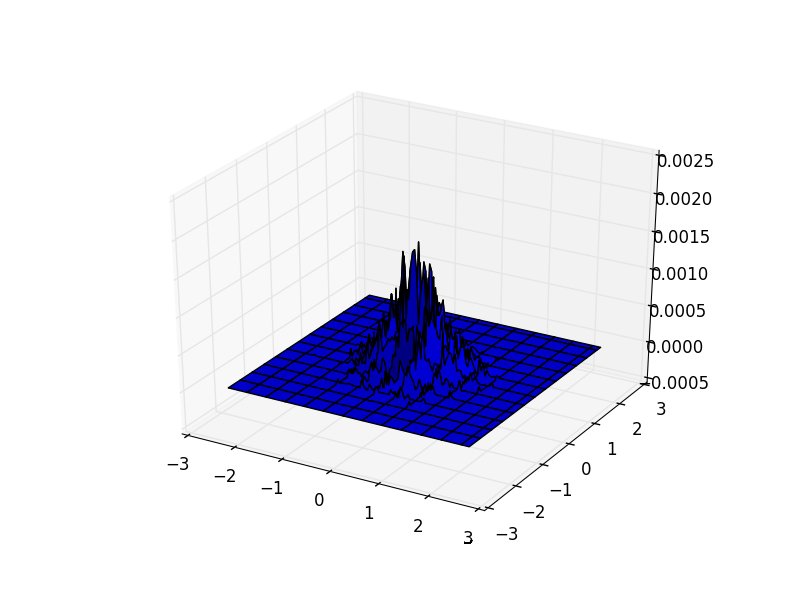
\includegraphics[width=.8\linewidth]{vorticity_distribution_for_14400_particles.png}
  		\caption{vorticity distribution for 14400 particles}
  		\label{fig:144}
	\end{subfigure}
	\label{fig:Question 1a}
  \caption{vorticity distribution for 12100 \& 14400 particles}

\end{figure}

\begin{figure}[h]
	\centering
	\begin{subfigure}[h]{.5\textwidth}
  		\centering
  		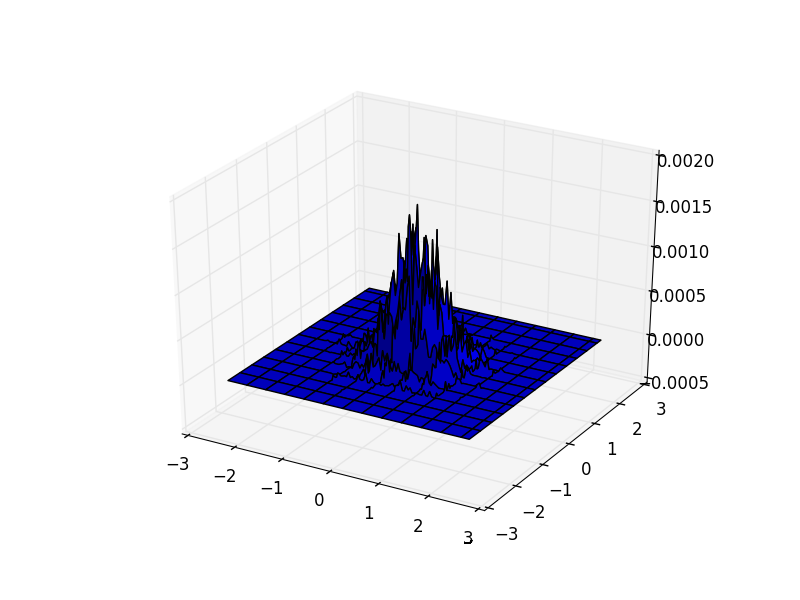
\includegraphics[width=.8\linewidth]{vorticity_distribution_for_16900_particles.png}
  		\caption{vorticity distribution for 16900 particles}
  		\label{fig:169}
	\end{subfigure}%
	\begin{subfigure}[h]{.5\textwidth}
  		\centering
  		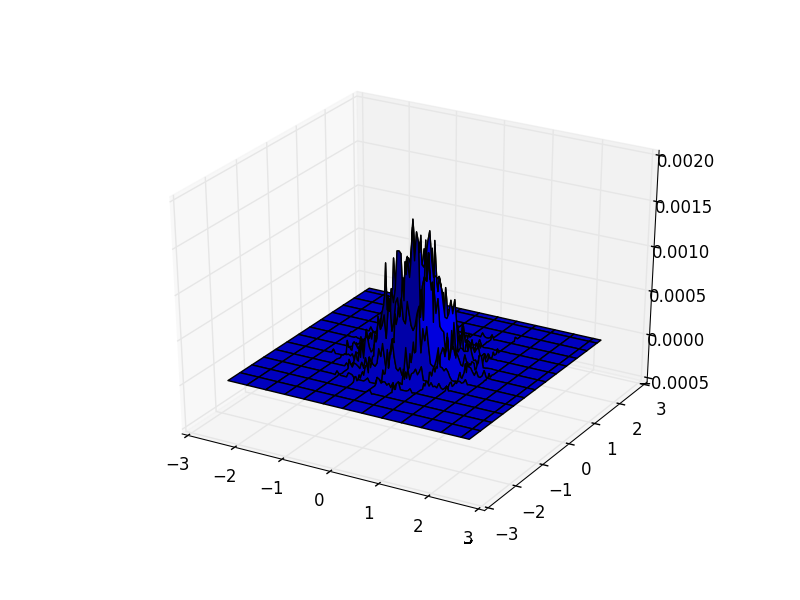
\includegraphics[width=.8\linewidth]{vorticity_distribution_for_19600_particles.png}
  		\caption{vorticity distribution for 19600 particles}
  		\label{fig:196}
	\end{subfigure}
	\label{fig:Question 1a}
  \caption{vorticity distribution for 16900 \& 19600 particles}

\end{figure}

\begin{figure}[h]
	\centering
	\begin{subfigure}[h]{.5\textwidth}
  		\centering
  		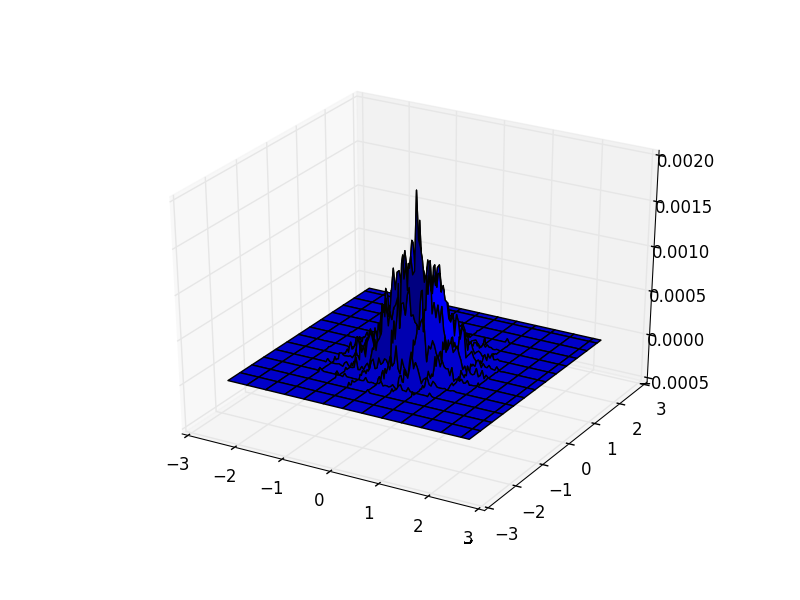
\includegraphics[width=.8\linewidth]{vorticity_distribution_for_22500_particles.png}
  		\caption{vorticity distribution for 22500 particles}
  		\label{fig:225}
	\end{subfigure}%
	\begin{subfigure}[h]{.5\textwidth}
  		\centering
  		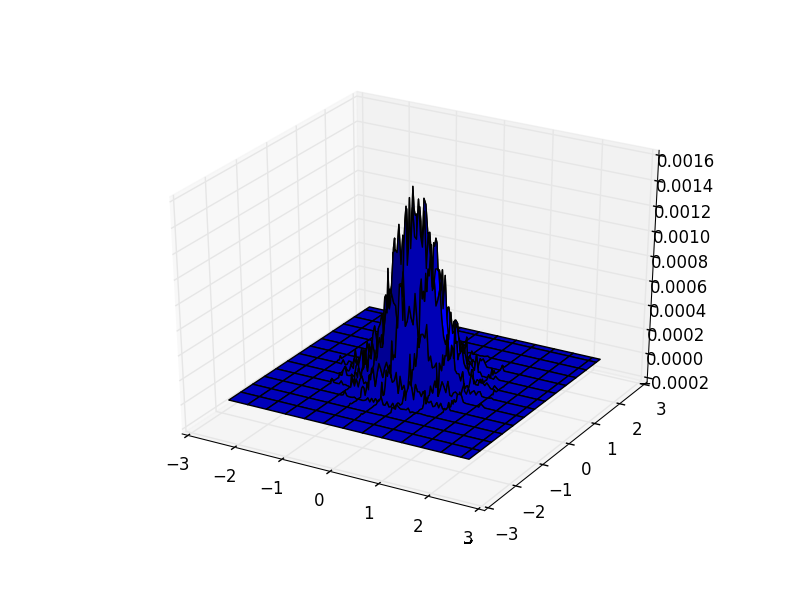
\includegraphics[width=.8\linewidth]{vorticity_distribution_for_27000_particles.png}
  		\caption{vorticity distribution for 27000 particles}
  		\label{fig:270}
	\end{subfigure}
	\label{fig:Question 1a}
  \caption{vorticity distribution for 22500 \& 27000 particles}

\end{figure}

\begin{figure}[h]
	\centering
    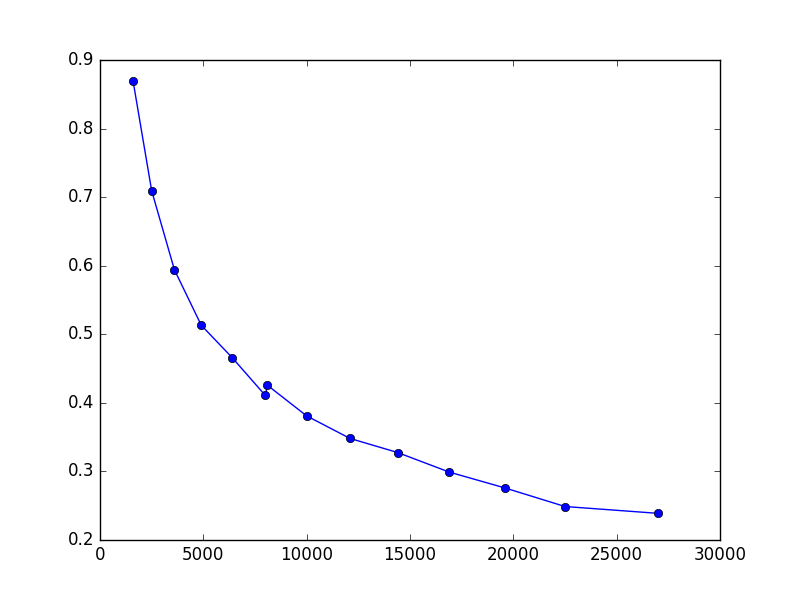
\includegraphics[width = 0.8\linewidth]{Error_for_different_no_of_particles.png}
    \caption{Error for different no of particles}
    \label{fig:err}

	
\end{figure}


\end{document}

